\documentclass{article}
\usepackage[T1]{fontenc}
\usepackage{lmodern}
\usepackage{graphicx}
\usepackage{amsmath,amssymb}
\usepackage[a4paper,margin=2cm]{geometry}
\usepackage[absolute,overlay]{textpos}
\setlength{\TPHorizModule}{1mm}
\setlength{\TPVertModule}{1mm}
\usepackage[indonesian]{babel}
\usepackage{hyperref}
\setlength{\emergencystretch}{2em}
% unit: Halaman 7

\begin{document}

% === Halaman 7 (llm) ===

\vspace{196.02mm}

\begin{itemize}
    \item Hasil penjumlahan $R_{i-1}$ dengan $K_i$ menghasilkan luaran yang panjangnya 32 bit.
    \item Luaran ini dibagi menjadi 8 bagian yang masing-masing panjangnya 4 bit.
    \item Setiap 4 bit masuk ke dalam kotak $S$ untuk proses substitusi. Empat bit pertama masuk ke dalam kotak $S$ pertama, 4 bit kedua masuk ke dalam kotak $S$ kedua, demikian seterusnya.
    \item Hasil substitusi setiap kotak $S$ adalah 4 bit. $GOST$ memiliki 8 buah kotak $S$, setiap kotak berisi 16 buah elemen nilai. Setiap kotak berisi permutasi angka 0 sampai 15.
\end{itemize}

\vspace{10mm}

Keterangan: $\square$ adalah operator penjumlahan dalam modulo $2^{32}$

% deskripsi: Diagram blok fungsi enkripsi GOST yang menunjukkan struktur Feistel dengan komponen fungsi f, substitusi kotak-S, pergeseran sirkuler, dan operasi modulo 2^32.
% bbox normalisasi: [0.5400, 0.1600, 0.9900, 0.8200]
\begin{textblock*}{94.50mm}(113.40mm,47.52mm)
\noindent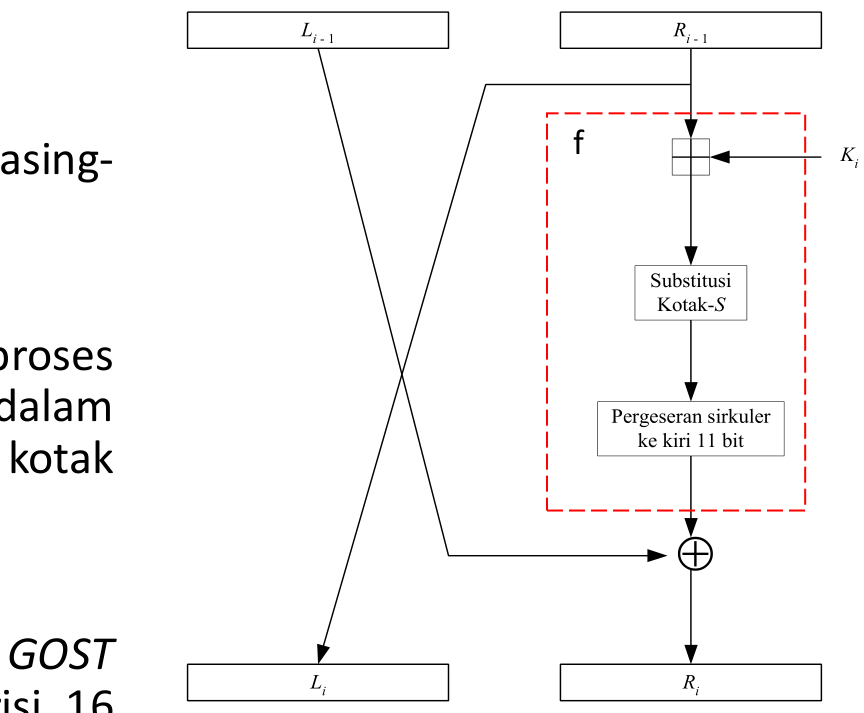
\includegraphics[width=94.50mm,height=196.02mm]{../../images/llm/page_007_img_01.png}%
\end{textblock*}

\end{document}
